\documentclass[class=report, crop=false, 12pt,a4paper]{standalone}
\usepackage{enumitem}
\usepackage{multicol}
\usepackage{etoolbox}
\AtBeginEnvironment{quote}{\singlespacing\small}
\usepackage{setspace}
\onehalfspacing
\usepackage{graphicx}
\usepackage{float}
\usepackage{siunitx}
\sisetup{detect-all}
\begin{document}
\section{Second Law of Thermodynamics}
First, let us remind ourselves of the first law of thermodynamics and some of its limitations. 
\begin{quote}
  \begin{center}
    Energy can neither be created or destroyed during a process; it can only change forms.
  \end{center}
\end{quote}
A certain energy balance will hold when a system undergoes change or a thermodynamic process.
\begin{itemize}[noitemsep]
  \item But does not give information on whether the change of state or the process is at all feasible or not.
  \item It cannot indicate whether a metallic bar of uniform temperature can spontaneously become warmer at one end and cooler at the other.
  \item However, if that process did occur, all that law can state is that the energy gained at one end would exactly equal the energy lost at the other.
\end{itemize}
\subsubsection{Introduction to the second law}
The second law of thermodynamics provides the criterion as to the \emph{probability} of various processes. 
\begin{quote}
  \begin{center}
    Spontaneous processes in nature occur only in one direction. 
  \end{center}
\end{quote}
Heat flows from a body at high temperature to a body at low temperature; water always flows downwards etc. The spontaneity of the process is due to finite driving potential, sometimes called 'force' or 'cause', e.g. a temperature or concentration gradient or an electric potential. What happens as a result of this finite driving potential is called the 'flux' or the 'current' or the 'effect' (heat transfer, mass transfer, flow of electric current). This directional law puts a limitation on energy transformation other than that imposed by the first law. The second law also asserts that energy has \emph{quality} as well as \emph{quantity.} The first law is concerned with the quantity of energy and the transformations of energy from one form to another, with no regard to its quality. 
\subsection{Qualitative difference between heat and work}
There is also a qualitative difference between heat and work. Energy supplied as work can be completely converted to heat, e.g. paddle wheel work on a liquid in an adiabatic vessel. However, the complete conversion of heat into work is not possible, thus making heat and work not completely interchangeable forms of energy. Also, we considered the problem of a simple steam power plant and by using the Steady Flow Energy Equation (i.e. first law) and the properties of steam, were able to calculate the work done and heat transfers for individual components. However, we are not yet able to understand ways of improving steam engine efficiency.

The second law is based on experimental observation and was the result of the question, 'how efficient can one make a steam engine?' From now we will start by considering engines and define them with the precision that thermodynamics requires. The sort of steam engines we shall discuss are heat devices in boxes with no fluid entering or leaving but with just heat and work crossing the boundaries.
\subsection{Thermodynamic cycles and thermal reservoirs}
Thermodynamic cycles consist of a system, a cold reservoir and a hot reservoir. Reservoirs are regions outside a system that are so large that their intensive properties remain constant. Thermal reservoirs are bodies that exchange an infinite amount of heat with the system. The temperature of a thermal reservoir never changes. For example: Earth's atmosphere, large bodies of water, vapour condensing at a constant pressure. A \emph{heat sink} absorbs heat energy. A \emph{heat source} transfers energy to the system.
\subsection{Heat engine}
A heat engine (or Cyclic Heat Power Plant - CHPP) is a continuously operating thermodynamic system at the boundary of which there are heat and work transfers.
Notes:
\begin{itemize}[noitemsep]
  \item 'Continuously operating' means that the state of the system exhibits only periodic (cyclic) changes.
  \item The heat engine is a thermodynamic system and so no matter crosses the boundary e.g. simple steam power plant and closed-cycle gas turbine plant.
\end{itemize}
As we know that heat transfer to work does not occur. However devices like heat engines have been created, which are special devices which are used to produce work from heat. All heat engines differ but can be characterised by the following: 
\begin{itemize}[noitemsep]
  \item They receive heat from a high temperature source (solar energy, oil furnace, nuclear reactor, etc.)
  \item They convert part of this heat to work (usually in the form of a rotating shaft.)
  \item They reject the remaining heat to a low temperature sink (the atmosphere, body of water, etc.)
  \item They operate on a cycle.
\end{itemize}
Diesel engines (Figure 3) (and internal combustion engines generally) are not heat engines (CHPP) because matter crosses its boundaries. A jet engine is also not a CHPP because matter, air, fuel and exhaust cross the boundary of the system.
\subsection{Steam power plant}
The work producing device that best suits this definition of a heat engine is the steam power plant, which is an external combustion engine.
\begin{enumerate}[noitemsep]
  \item Combustion takes place outside.
  \item Transferred to steam as heat.
  \item Passed through various devices that transfer its energy to work.
\end{enumerate}
Figure 4 shows a simplified diagram of a steam plant. From this we can see that \(W_{\textrm{net out}} = W_{\textrm{out}} - W_{\textrm{in}}\) (\si{\kilo\joule}). Considering that the change in internal energy is zero for cycles, we can derive, \(W_{\textrm{net out}} = Q_{\textrm{in}} - Q_{\textrm{out}}\) (\si{\kilo\joule}).
\subsection{Thermal efficiency of direct engines/steam power plants}
For heat engines, the desired output is the net work output and the required input is the amount of heat supplied to the working fluid. Thus the thermal efficiency is expressed as:
\[ \textrm{Thermal efficiency} = \frac{\textrm{Net work output}}{\textrm{Total heat input}} \]
\[ \eta = \frac{W_{\textrm{net out}}}{Q_{\textrm{in}}} \]
\[ \eta = 1 - \frac{Q_{\textrm{out}}}{Q_{\textrm{in}}} \]
Since cyclic devices at practical interest operate between a high temperature \(T_H\) and a low temperature medium \(T_L\), we define these two quantities:
\begin{itemize}
  \item {\(Q_H =\)} magnitude of heat transfer between the cyclic device and the high temperature medium \(T_H\).
  \item {\(Q_L =\)} magnitude of heat transfer between the cyclic device and the low temperature medium \(T_L\).
\end{itemize}
Thus, the previous equations can be written as follows:
\[ W_{\textrm{net out}} = Q_H - Q_L \]
\[ \eta = 1 - \frac{Q_L}{Q_H} \]
Thermal efficiencies of work producing devices are relatively low. Ordinary spark ignition automobile engines have a thermal efficiency of about 25\%. Gas steam power plants reach only 60\%.
\subsection{Can we save \(Q_{out}\)?}
In a steam power plant, the condenser is the device where large quantities of waste heat is rejected to rivers, lakes or the atmosphere. One may ask, can we not save all this waste energy? The answer is a firm \emph{no}. Without a heat rejection process in the condenser, the cycle cannot be completed. Cyclic devices such as steam power plants cannot run continuously, unless the cycle is completed.
\subsection{The Kelvin-Planck statement}
The Kelvin-Planck statement of the second law of thermodynamics is expressed as follows:
\begin{quote}
  \begin{center}
    It is impossible for any device that operates on a cycle to receive heat from a single reservoir and produce a net amount of work.
  \end{center}
\end{quote}
A heat engine must exchange heat with a low temperature sink as well as a high temperature source to keep operating. This implies that it is impossible to build a heat engine that has a thermal efficiency of 100\%. Complete conversion of heat into work is \emph{not possible.} This is contrary to the fact that 100\% of work can be transferred to heat. This is the directional implication of the second law. This is not due to frictional/non-adiabatic effects. It is a \emph{necessity.}

Proof on page 128 of Cengel (insert edition.)
\subsection{Refrigerators and heat pumps}
From experience, heat always from from high temperature to low temperature. These reverse process, however, cannot occur by itself. This reverse process requires special devices called refrigerators. Refrigerators are cyclic devices and the working fluid is called a refrigerant. A frequently used refrigeration cycle is the 'vapour-compression refrigeration cycle.' This involves a compressor, a condenser, an expansion valve and an evaporator.
\subsection{Coefficient of performance}
The efficiency of a refrigerator is called the coefficient of performance (COP), denoted by \(\textrm{COP}_R\). The objective of a refrigerator is to: remove heat from the refrigerated space by being provided with a work input \(W_{\textrm{net in}}\). Thus:
\[ \textrm{COP}_R = \frac{Q_L}{W_{\textrm{net in}}} = \frac{\dot{Q}_L}{\dot{W}_{\textrm{net in}}} \]
Also, since \(W_{\textrm{net in}} = Q_{\textrm{in}} - Q_L\)
\[ \textrm{COP}_R = \frac{Q_L}{Q_H-Q_L} \]
\[ \textrm{COP}_R = \frac{1}{\frac{Q_H}{Q_L} - 1}\]
COP can also be greater than unity. This means the heat removed can be greater than the work input. Whereas thermal efficiency can never be greater than 1. 


\subsection{Reversed heat engine}
The definition of a heat engine says nothing about the direction of heat and work transfers. Thus, this makes a domestic refrigerator a heat engine. The domestic refrigerator consists of: 
\begin{multicols}{2}
  \begin{itemize}[noitemsep]
    \item Condenser.
    \item Vapour compressor.
    \item Evaporator.
    \item Throttle.
  \end{itemize}
\end{multicols}
Compare this to other heat engines e.g. steam/gas turbine power plants, where the component roles are reversed.
\begin{multicols}{2}
  \begin{itemize}[noitemsep]
    \item Boiler $>$ Condenser.
    \item Turbine $>$ Compressor.
    \item Condenser $>$ Evaporator.
    \item Pump $>$ Throttle.
  \end{itemize}
\end{multicols}
\section{Reversibility}
\section{Entropy}
\section{Figures}
\begin{figure}[H]
  \begin{center}
    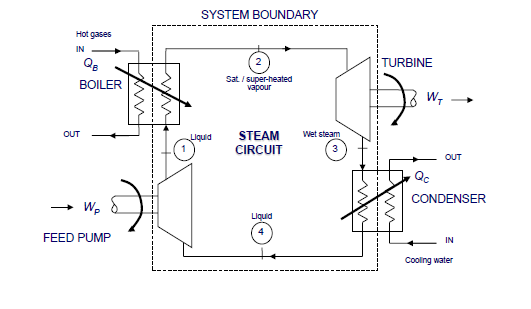
\includegraphics[width = \textwidth]{../img/SimpleSteamPP}
    \caption{A simple steam power plant}
  \end{center}
\end{figure}
\begin{figure}[H]
  \begin{center}
    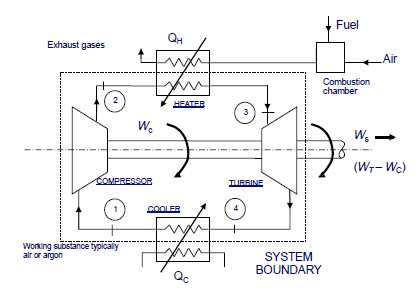
\includegraphics[width = \textwidth]{../img/ClosedCycleGasPP}
    \caption{A closed cycle gas power plant}
  \end{center}
\end{figure}
\begin{figure}[H]
  \begin{center}
    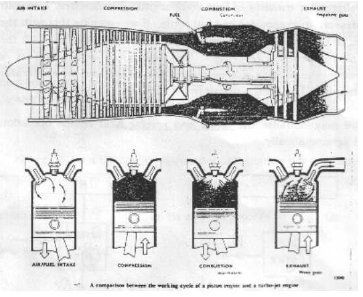
\includegraphics[width = \textwidth]{../img/DieselEngine}
    \caption{A diesel engine}
  \end{center}
\end{figure}
\begin{figure}[H]
  \begin{center}
    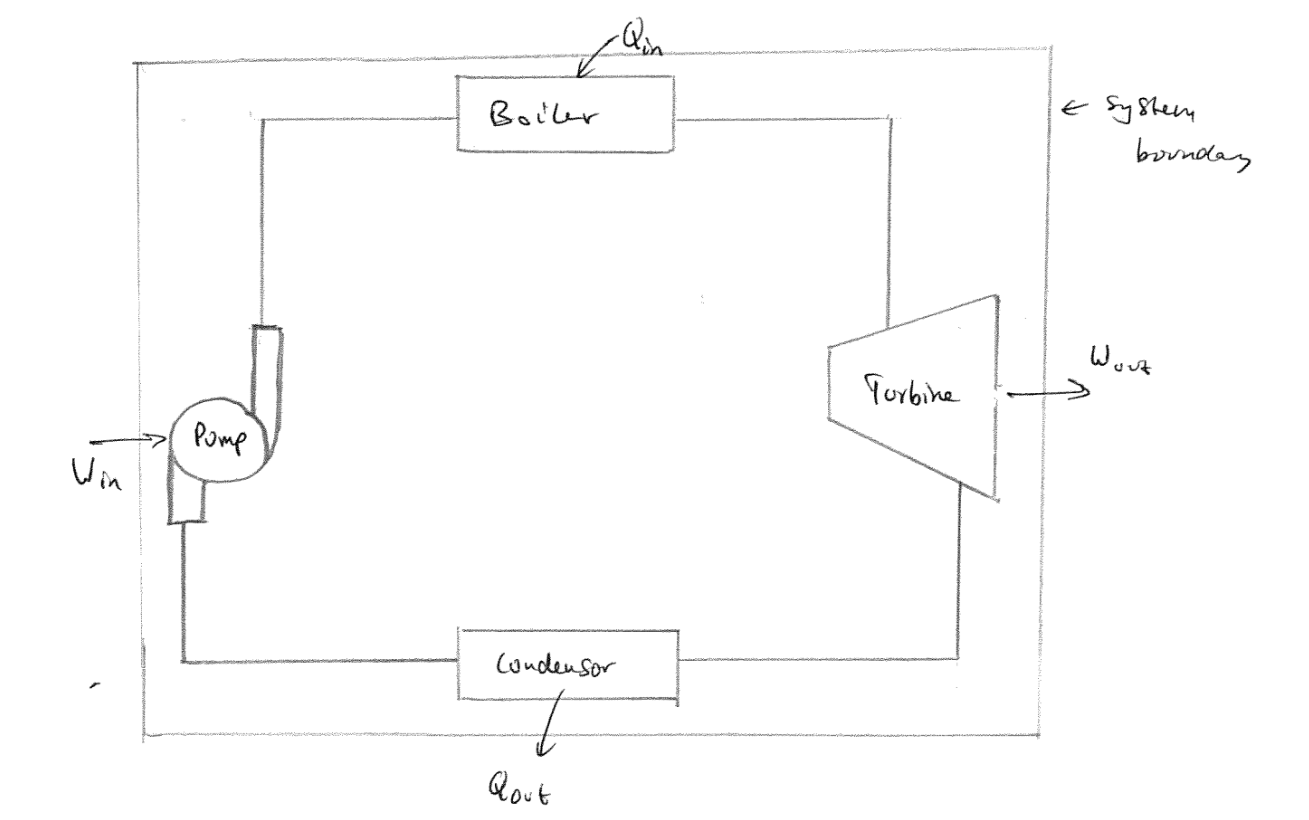
\includegraphics[width = \textwidth]{../img/SteamPowerPlantDiagram}
    \caption{A diesel engine}
  \end{center}
\end{figure}
\begin{figure}[H]
  \begin{center}
    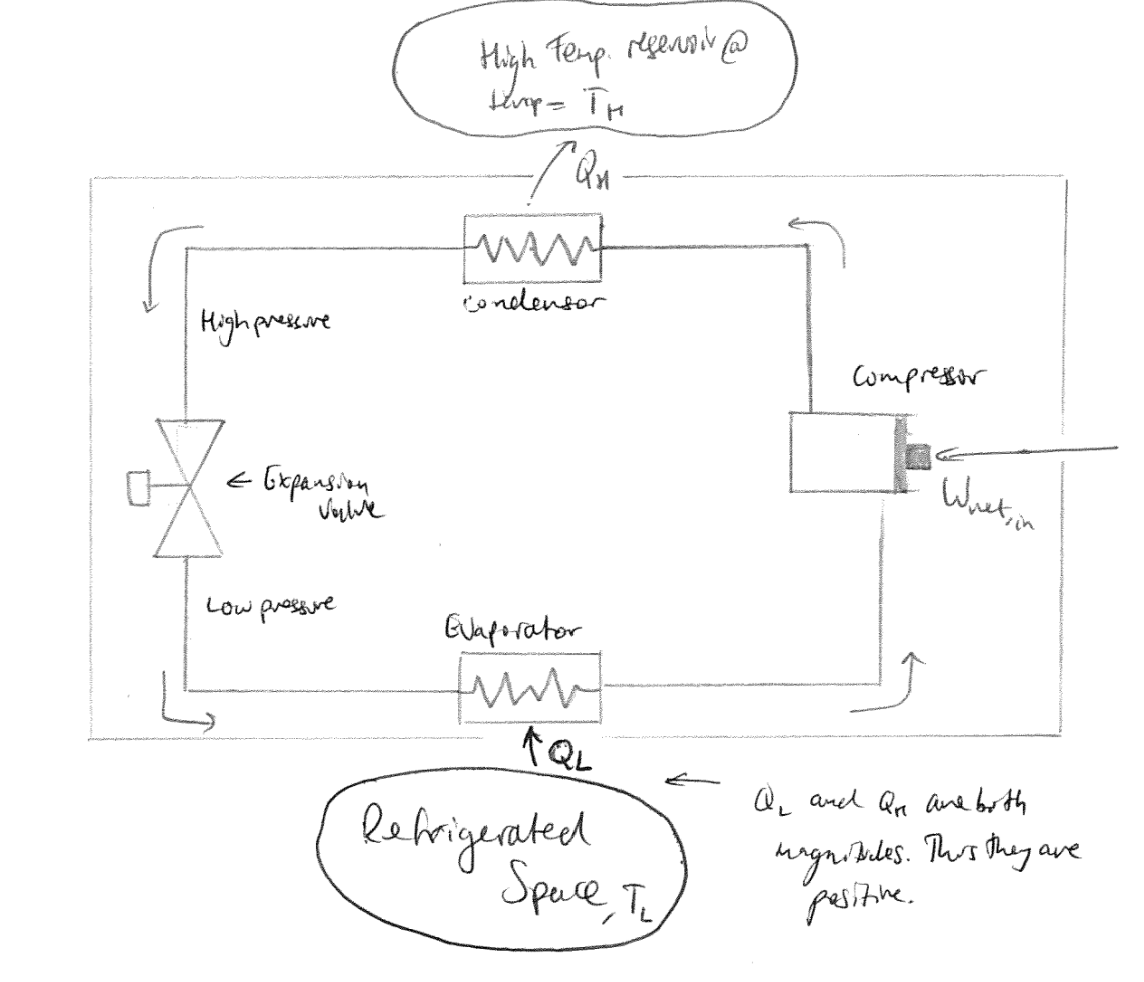
\includegraphics[width = \textwidth]{../img/RefrigerationCycle}
    \caption{A diesel engine}
  \end{center}
\end{figure}
\end{document}